
\chapter{Implementation and Results}
\section{Implementation}

\subsection{Libraries and Frameworks}
The execution of the classroom ventilation optimization system is built upon a robust combination of Python libraries and embedded tools, each serving a distinct role within the sensor data processing, model training, and real-time inference pipeline. The integrated components are outlined as follows:
\subsubsection{Python Libraries}
\begin{itemize}
    \item serial: Enables serial communication between the Raspberry Pi and Arduino, handling data transmission and reception for sensor readings and control commands.
    \item numpy: Provides support for large, multi-dimensional arrays and matrices, essential for data processing and mathematical operations in sensor data analysis and LSTM model operations.
    \item tensorflow: The core deep learning framework used to implement the LSTM neural network model, providing both the model architecture and training capabilities for environmental prediction.
    \item pandas: Handles data manipulation and analysis, particularly useful in loading and preprocessing the training dataset and managing time-series environmental data.
    \item sklearn.preprocessing: Contains the MinMaxScaler class used for normalizing sensor data and ensuring consistent scale across different environmental parameters.
    \item logging: Implements comprehensive system logging functionality, tracking system operations, errors, and model performance metrics for debugging and monitoring.
    \item datetime: Manages time-related operations and timestamps for data collection, helping track temporal patterns in environmental conditions.
    \item json: Handles JSON data formatting for configuration storage and cloud communication, particularly for classroom metadata and model parameters.
    \item requests: Manages HTTP communications for cloud data upload to ThingSpeak and model synchronization operations.
    \item RPi.GPIO: Controls Raspberry Pi's GPIO pins for interfacing with the LCD display and other hardware components.
    \item RPLCD.gpio: Specifically handles LCD display operations, providing methods for showing real-time environmental data and system status.
\end{itemize}
\begin{figure}[h!]
		\centering
	\includegraphics[width=0.8\textwidth]{Pictures/modules.png}
		\caption{Module Imports for Sensor Integration, Data Processing, and LSTM Model Execution}
\end{figure}
\subsubsection{Arduino Libraries}
\begin{itemize}
    \item LiquidCrystal.h: Manages the LCD display on the Arduino side, providing functions for displaying sensor readings and status information.
    \item DHT.h: Interfaces with the DHT11 temperature and humidity sensor, handling raw sensor data collection and basic processing.
\end{itemize}
Each of these libraries is responsible for the project's functionality, starting from data collecting and processing and ending with its display and communication. The blending of these libraries makes it possible to create an integrated environmental monitoring and control system.

\subsection{Sensor Data Collection and processing}
\subsubsection{Data Extraction}
Sensor Data Reading and Collection Process

The environmental monitoring system implements a systematic approach to sensor data collection, operating on a precisely timed cycle to gather comprehensive classroom environmental data. Each Arduino unit manages a specific sequence of sensor readings, ensuring efficient data collection while maintaining accuracy across all parameters.

The data collection cycle begins with the DHT11 sensor readings. Every 2 seconds, the system first samples temperature data, followed immediately by humidity measurements. The DHT11 sensor's digital interface requires specific timing protocols, with a minimum 2-second interval between readings to ensure accurate measurements. Temperature readings are captured within the 0-50°C range with ±2°C accuracy, while humidity measurements span 20-90\%. These environmental parameters form the baseline for classroom condition assessment.

Following the temperature and humidity readings, the system queries the MQ135 sensor for CO2 concentration levels. The MQ135 sensor requires a warm-up period of approximately 20 seconds after initial power-up to ensure accurate readings. Once operational, it continuously monitors CO2 levels between 400ppm to 2000ppm. The sensor's analog output is converted through the Arduino's ADC (Analog to Digital Converter) to provide precise CO2 concentration values.

Simultaneously with environmental parameter monitoring, the IR sensor pairs at classroom doorways continuously track occupancy changes. These sensors operate on an interrupt-driven basis, ensuring no movement events are missed regardless of the main sampling cycle. Each doorway is equipped with two IR sensors, enabling directional detection (entry vs. exit). The system maintains separate counters for incoming and outgoing movements, updating the occupancy count in real-time.

The Arduino compiles these readings into a structured data string following the format 'aXXbYYcZZdWWeVVfUUg\n', where:
1. XX: Current temperature reading
2. YY: Current humidity value
3. ZZ: CO2 concentration level
4. WW: Current inside person count
5. VV: Outside person count
6. UU: Calculated KPIv value

This data string is transmitted to the Raspberry Pi every 2 seconds through the USB serial connection (ttyS0 or ttyS1) at 9600 baud rate. The timing of these transmissions is carefully managed to prevent data collision between the two classroom units. Each transmission includes error checking mechanisms to ensure data integrity.

The Raspberry Pi receives these data strings from both classroom units, implementing immediate validation checks before processing. The DataHarmonizer class maintains separate buffers for each classroom, applying a 5-reading moving window to smooth variations and detect anomalies. This harmonization process runs continuously, ensuring that the LSTM model always has access to reliable, current environmental data for pattern recognition and prediction.

This systematic approach to sensor data collection and initial processing ensures comprehensive environmental monitoring while maintaining data reliability. The carefully timed reading sequence and structured data format enable efficient processing and analysis, forming the foundation for the system's environmental control capabilities.
%The data extraction process for this project functions on various levels, integrating real-time sensor data gathering and advanced processing and analysis mechanisms. On the hardware level, the system draws environmental information via an array of sensors: a DHT11 sensor gathers temperature and humidity information, a specialized CO2 sensor tracks air quality readings, and two infrared beam sensors monitor room occupancy. These sensors continually sample their corresponding parameters, the Arduino microcontroller being the central point of data collection, where it gathers and first processes this raw sensor data.
%The system deploys a comprehensive data harmonization policy via the DataHarmonizer class, which filters raw sensor data coming in to remove noise and detect anomalies. Harmonization is based on a moving window strategy (usually 5 readings) that smooths sensor variations and flags outliers. Statistical analysis, including z-score determinations, is used by the harmonizer to flag and correct anomalous readings that are substantially different from current trends. Furthermore, the harmonizer adds classroom-specific context by standardizing occupancy against room capacity and including time-based features like hour-of-day, which improves the system's capability to identify patterns in environmental variations.
%The data extracted is organized into extensive sequences for the LSTM neural network model. Each sequence integrates several environmental parameters (temperature, CO2 levels, humidity, occupancy) with calculated metrics such as the Ventilation Key Performance Indicator (KPIv). The MinMaxScaler is used by the system to normalize all the input features, keeping the scale uniform across various parameters and enhancing model training effectiveness. The sequence creation process maintains a temporal aspect, with each sequence containing 10 consecutive readings, allowing the model to learn patterns in environmental changes over time.
%Data transmission happens on multiple channels. The Arduino transmits formatted data strings to the Raspberry Pi at 5-second intervals, encoding all of the sensor measurements and calculated measures in a precise format. Data is then received by the Python-based monitoring program, which holds individual data buffers for each room. The system also employs cloud synchronization using ThingSpeak, posting processed data on a regular schedule (usually once per hour) for remote examination and analysis.
%The project features a state-of-the-art data quality management system. The Data Harmonizer class not only processes input data but also enforces data integrity through a number of mechanisms. It takes care of missing values by intelligent interpolation, eliminates physical impossibilities (such as negative occupancy numbers), and preserves temporal consistency of the data stream. The system also performs data validation checks at multiple levels, ranging from simple range checking of sensor values to more sophisticated validation of derived measures such as KPIv calculations.
For training models, the system keeps historical buffer data, capping each classroom at 1000 samples to balance memory and model accuracy. Feature engineering during data extraction is also involved in generating derived features like occupancy ratios, ventilation efficiency metrics, and trend indicators. These engineered features blend raw sensor data with domain knowledge regarding indoor air quality dynamics to improve the predictive power of the model. The data processing and extraction pipeline of the system ends with the production of an integrated environmental monitoring system that not only gathers data but also transforms.

The process begins with the systematic loading of environmental data from structured CSV files, which serve as historical repositories of classroom conditions. The system focuses on five critical environmental metrics that paint a comprehensive picture of the indoor environment. CO2 levels are monitored as a primary indicator of air quality and ventilation effectiveness, providing crucial insights into the room's breath ability. Temperature readings help maintain optimal learning conditions, while humidity measurements ensure comfort and prevent conditions conducive to mold growth. The occupancy tracking provides real-time data about room usage patterns, essential for ventilation optimization. Time data is carefully parsed to maintain the temporal context of all measurements, enabling the system to identify patterns across different times of day and days of the week. Each data point is timestamped with precision, ensuring that the chronological sequence of environmental changes is preserved. This temporal alignment is crucial for understanding how classroom conditions evolve throughout the day and helps in predicting future trends. The system employs sophisticated parsing algorithms to handle various timestamp formats, ensuring consistency across all data entries.

\subsubsection{Data Cleaning}
The data cleaning phase represents a critical step in ensuring data reliability and consistency. When dealing with real-world sensor data, missing readings are an inevitable challenge that must be addressed systematically. The system employs a sophisticated two-pronged approach to handle these gaps. First, forward filling is applied, where missing values are populated with the last known valid reading. This approach is based on the assumption that environmental conditions typically change gradually, making the previous reading a reasonable estimate for small gaps. For cases where forward filling isn't sufficient, backward filling is employed as a secondary strategy, looking ahead to the next valid reading to fill gaps at the beginning of the dataset. This dual-filling strategy ensures continuity in the data while maintaining realistic value ranges. Beyond handling missing data, the system performs comprehensive validation checks to ensure data completeness and consistency. This includes verifying that sensor readings fall within physically possible ranges, detecting and handling outliers that might indicate sensor malfunctions, and ensuring that the temporal sequence of readings remains logical. Invalid measurements, such as physically impossible temperature readings or corrupted sensor data, are identified and removed through carefully crafted validation rules. This cleaning process maintains the integrity of the dataset while preserving as much valid data as possible.
\\

\subsubsection{Data Transformation}
This process is the MinMaxScaler, which normalizes all measurements to a standardized 0-1 scale. This normalization is crucial because different environmental metrics operate on vastly different scales - CO2 levels might range from 400 to 2000 ppm, while temperature might range from 18 to 30 degrees Celsius. By bringing all measurements into the same scale, the system ensures that no single metric dominates the analysis simply due to its larger numerical range. Time data undergoes a special transformation to capture its cyclical nature. Instead of treating time as a linear progression, it's converted into a cyclical format that helps the model understand that 23:59 is actually closer to 00:00 than to 23:00. This transformation is crucial for capturing daily patterns in classroom usage and environmental changes. The system then creates sequences of 10 timesteps, providing the LSTM model with enough historical context to make accurate predictions while maintaining computational efficiency.
\subsection{IoT Hardware Architecture}
\begin{figure}[h]
    \centering
    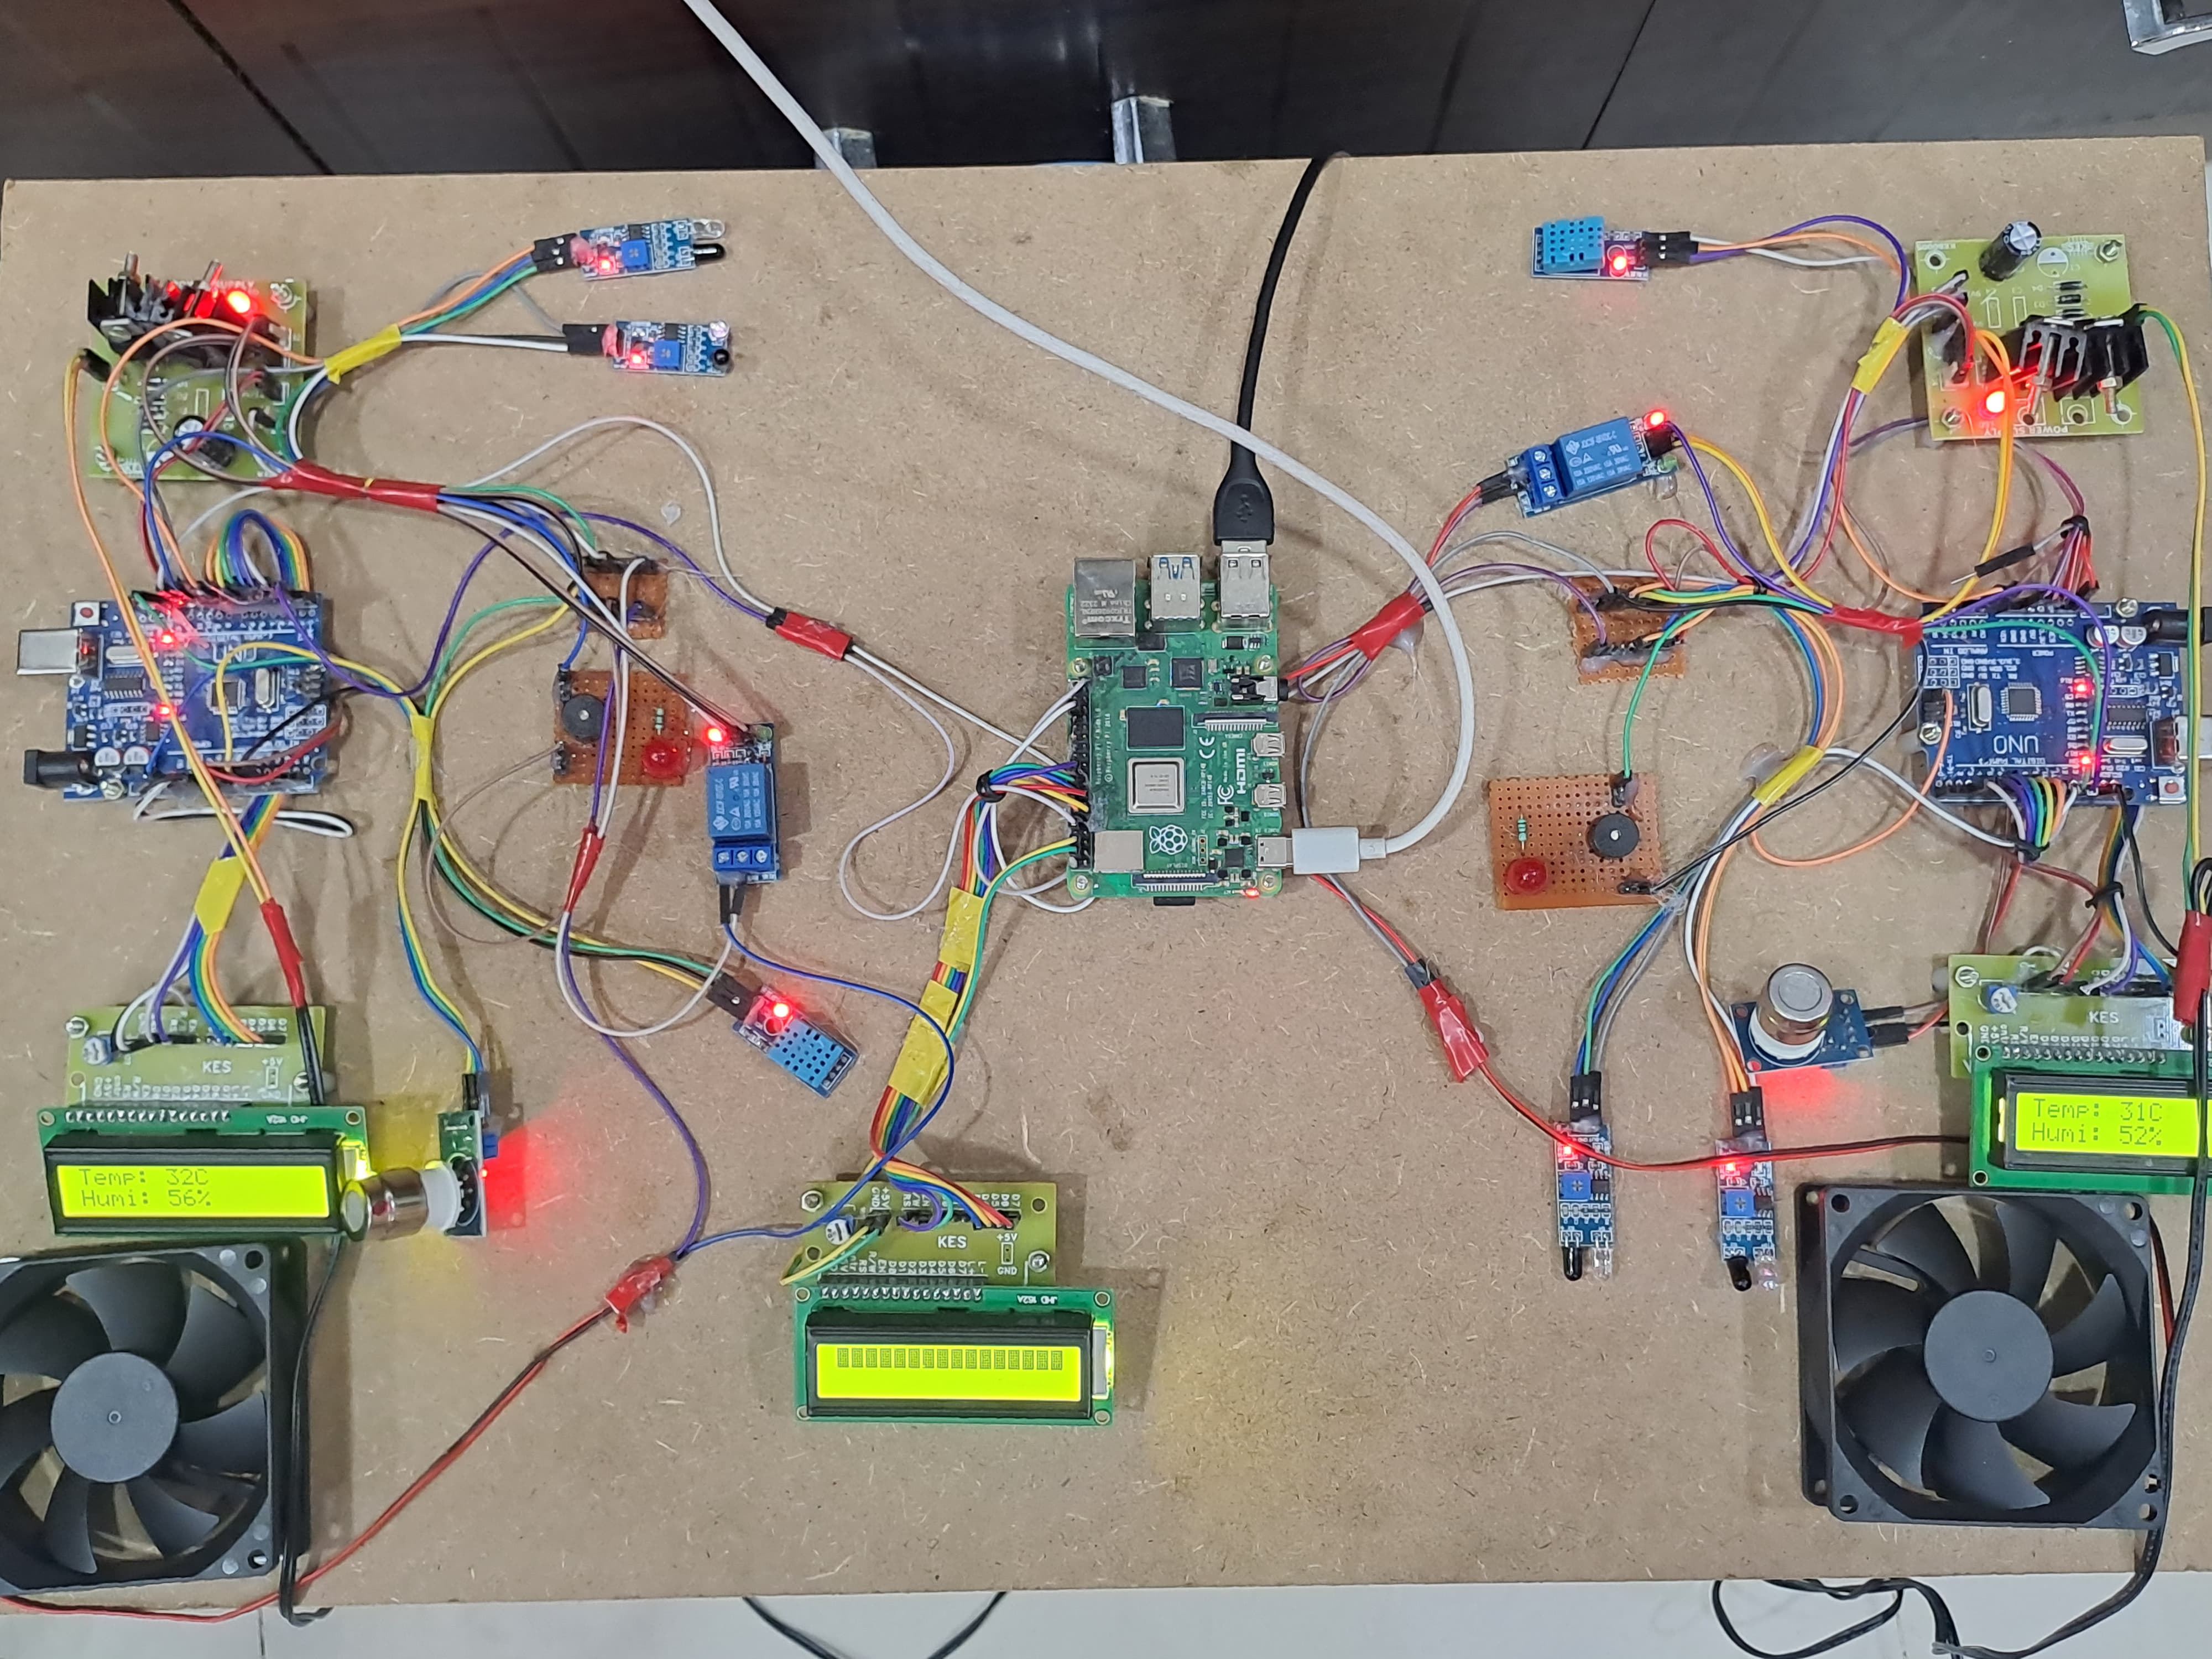
\includegraphics[width=0.8\textwidth]{Chapters/kit.jpg.jpeg}
    \caption{Complete Edge-Based IoT Hardware Architecture for Classroom Ventilation Optimization}
    \label{fig:augmentation}
\end{figure}

The hardware setup shown in the image(\ref{fig:augmentation}) brings to life a smart and practical solution for monitoring air quality in real-time across two different classrooms. The main idea behind this system is simple yet powerful: measure CO₂ levels and track how many people are in each room, then use that information to predict indoor air quality and figure out which room is healthier and more comfortable to use at any given moment. It’s like giving classrooms their own environmental intelligence—and it all comes together with a thoughtful mix of sensors, microcontrollers, and real-time decision-making hardware. At the center of this system is a Raspberry Pi 4, which acts like the brain of the operation. It handles the heavy lifting, making smart decisions based on incoming data. On either side of it are two Arduino Uno boards, each responsible for one classroom. These boards are directly connected to various sensors and serve as the first responders, collecting data from their surroundings and passing it on to the Raspberry Pi.

Each Arduino is connected to a DHT11 sensor that reads the room’s temperature and humidity, a set of IR sensors placed near what would be the room entrances to detect when people walk in or out, and a CO₂ gas sensor that continuously monitors the air quality. The IR sensors are arranged in pairs, allowing the system to count people moving in both directions, which helps determine how many occupants are currently in the room. The DHT11 is strategically placed to get a reliable reading of the room’s overall temperature and moisture, while the CO₂ sensor gives constant updates on the amount of carbon dioxide in the air—a key indicator of how fresh or stale the environment is. The two Arduinos send this real-time data to the Raspberry Pi using USB serial communication. Once the data arrives, the Raspberry Pi takes over. It uses a pre-trained LSTM (Long Short-Term Memory) model—a type of AI that’s really good at understanding time-based data—to predict how the CO₂ levels are likely to change in the near future. This allows the system to respond not just to what’s happening now, but also to what’s about to happen—kind of like having a weather forecast for classroom air quality.

To make this system interactive and easy to use, LCD screens are placed below each sensor cluster. These display live readings of temperature and humidity so anyone nearby can immediately see the environmental status of the room. Cooling fans, relays, and buzzers are also part of the setup. When the system predicts that CO₂ levels are getting too high, it can automatically turn on the fan to improve air circulation or trigger a buzzer and LED to alert users of poor air quality.

Altogether, this hardware kit(\ref{fig:augmentation}) isn’t just a tech experiment—it’s a complete, real-world prototype of a smart classroom management system. It’s designed to help students and teachers breathe easier and make better choices about which room to use. By combining edge-level sensing with fog-level AI processing and simple output components, it creates a closed-loop system that’s proactive, responsive, and built for smarter, healthier classrooms. This approach can easily be scaled to entire school buildings or campuses, offering an energy-efficient, health-first solution for the future of indoor learning environments.

\subsection{Arduino code}
Arduino sketch initializes key components and constants for monitoring CO₂ levels, temperature, and occupancy within a classroom using sensors and an LCD display. It includes necessary libraries for the LCD (LiquidCrystal.h) and the DHT11 temperature and humidity sensor (DHT.h). Several constants are defined, such as CO2 THRESHOLD and TEMP THRESHOLD, which act as benchmarks for detecting elevated CO₂ concentration and temperature. An ALARM\_CO2 value is also set to trigger an alert when dangerous CO₂ levels are reached. Additionally, constants like BASE\_CO2 and CO2\_PER\_PERSON are used to estimate the number of people in the room based on CO₂ readings. The system connects various components to specific pins on the Arduino, including IR sensors for entry and exit detection, a CO₂ sensor, a relay, and a buzzer.

\subsubsection{Environmental Monitoring and Sensor Integration}
The environmental monitoring system serves as the backbone of the classroom management solution, integrating various sensor technologies to gain a complete understanding of indoor conditions. Central to this is the use of a DHT11 sensor to accurately measure temperature and humidity alongside an analog CO2 sensor to track air quality. The sensor integration is reliability oriented, utilizing advanced error checking and data validation techniques to provide precise readings in adverse conditions. The system repeatedly samples these environmental parameters, keeping rolling averages that smooth out any sensor oscillations and deliver stable, consistent measurements. This monitoring system not only gathers data, but it also actively processes and analyzes it in real-time, computing key performance indicators like the Ventilation Performance Indicator (KPIv). This computed metric considers several environmental factors to give a complete evaluation of room ventilation efficiency. The monitoring system also utilizes adaptive sampling rates, varying its measurement frequency in response to environmental factors and system load to maximize performance without impairing system responsiveness.

\subsubsection{Occupancy Tracking and Movement Detection}
The room occupancy counting system is one of the most advanced parts of the code and uses a state machine-based method to effectively count people in rooms. The system uses two IR beam sensors placed at the doorway to provide a directional detection system that can identify people moving into and out of the room. The state machine handles these beam breaks by cycling through five states: IDLE, IN\_FIRST, OUT\_FIRST, PASSING\_IN, and PASSING\_OUT. Every state change is monitored with care using debounce protection against false counts due to brief beam disruptions or environmental noise. Accurate counts are ensured in difficult conditions, including simultaneous people passing through and partial beam breaks. The occupancy tracking system has also advanced error recovery features, automatically identifying and curing possible counting errors by means of timeout mechanisms and state verification. This strong implementation provides stable occupancy information, which is important for ventilation control as well as environmental control. The system also cross-links occupancy information with CO2 measurements to confirm counting accuracy and identify possible anomalies in either measurement.


\subsubsection{Display Management and User Interface}
The display control system offers an advanced yet intuitive interface via a 16x2 LCD screen, using a rotating information system that rotates through various important statistics and notifications. The interface system is meant to optimize the limited display area while making all important information easily accessible to occupants of the room. The display rotation consists of three primary information screens: environmental conditions (temperature and humidity), air quality metrics (CO2 levels and KPIv), and occupancy information (current count and trends). The system uses smart display updates that focus on priority information during alert situations but keep regular information rotation in ordinary operation. The display management uses advanced formatting routines to provide concise, readable output independent of the data being presented. Priority display queue messages are assigned to alert messages, overriding rotation for a short time to provide instant visibility of the serious conditions. The system also has visual indications of system status, sensor health, and operation of the ventilation system, giving overall feedback regarding the environmental management system of the classroom.

\subsubsection{ Control Systems and Communication}
The control and communications component oversees the integration of environmental monitoring and active response systems. This involves advanced ventilation control by means of a relay system, which responds to various environmental factors such as CO2 levels, temperature, and occupancy. The system uses a predictive control algorithm that forecasts ventilation requirements based on trending data and existing conditions, instead of reacting solely to threshold violations. The communication system is always in a serial connection with a Raspberry Pi, using a stable protocol for data exchange that involves transmission of sensor data and parameter updates. The format of the data communication is properly designed to be reliable during reception and transmission, with error checking and validation incorporated in the protocol. The system also controls multiple output devices such as a buzzer for audio notification and the ventilation relay, with a priority-based control system providing suitable response to a number of different environmental situations. The control logic also contains advanced timing systems to prevent overcycling of the ventilation system without affecting the environmental control efficiency.
\subsection{LSTM-based Prediction and Control Implementation}

\subsubsection{ClassroomMonitor Class}
The ClassroomMonitor class is the mastermind of the entire smart classroom system, coordinating all the moving components like a conductor guiding an orchestra. It is the principal control center where all the key decisions regarding classroom environment management are taken. This class is responsible for opening and keeping communication channels with the Arduino sensors via serial ports, similar to having a direct line to field reporters who are collecting real-time data. It constantly gathers environmental data - temperature, humidity, CO2 levels, and occupancy levels - and processes this data to create a complete picture of classroom conditions.
What sets this class so smart is the fact that it can control a number of different classrooms at one time, and treat each classroom as an independent environment with distinct characteristics and needs. It is as if it has a supervisor for each class, but with all working through a single orchestrated system. The class executes high-level data sampling cycles, collecting sensor data constantly while keeping the system responsive and efficient. In terms of predicting and suggesting, the ClassroomMonitor behaves like a seasoned teacher who is well aware of when a classroom requires airing or when situations may turn stuffy. It is in touch with the physical world as well as the digital cloud all the time, so that important environmental information is not only gathered but also stored and analyzed to make long-term improvements.

\subsubsection{DataHarmonizer Class}
The DataHarmonizer class serves as a critical data preprocessing component in our classroom monitoring system, implemented to ensure data reliability and consistency across multiple sensor inputs. The implementation utilizes a 5-reading moving window approach, maintaining separate data buffers for each classroom to process temperature, humidity, CO2, and occupancy readings. This class is essential because raw sensor data often contains noise, outliers, or inconsistencies that could trigger false alerts or incorrect ventilation responses. The harmonization process begins when sensor data arrives from the Arduino units. Each data packet contains temperature, humidity, CO2 levels, and occupancy counts in a structured format. The harmonizer first adds this new data to a classroom-specific buffer, which maintains the five most recent readings. This buffer acts as a sliding window, automatically removing the oldest reading when a new one arrives, ensuring that the system always works with current environmental conditions. When processing the data, the harmonizer performs statistical analysis to identify potential outliers. It calculates the average and standard deviation of the recent readings for each environmental parameter. Any new reading that deviates significantly from these statistical measures (specifically, more than three standard deviations from the mean) is flagged as an outlier. Rather than simply discarding these outliers, the system replaces them with an average calculated from recent valid readings, ensuring continuity in the data stream while eliminating potentially erroneous values. The harmonizer also enriches the data by adding crucial contextual information. For occupancy data, raw counts are converted into meaningful percentages based on each classroom's maximum capacity. This standardization makes the data more comparable across different room sizes and more meaningful for the LSTM model's predictions. Additionally, the system incorporates temporal context by including the time of day as a normalized value, enabling the model to recognize and learn time-dependent patterns in classroom usage and environmental variations. This implementation has proven particularly valuable in handling common real-world sensor challenges. For instance, it effectively manages occasional DHT11 sensor misreadings, compensates for CO2 sensor warm-up periods, and smooths out temporary fluctuations in occupancy counts from the IR sensors. By maintaining separate processing buffers for each classroom while applying consistent harmonization logic, the system ensures reliable data quality across all monitored spaces while preserving the unique characteristics of each classroom's environment. The harmonized data provides a solid foundation for the LSTM model's predictions and the system's control decisions. By ensuring that only validated, contextually enriched data feeds into the prediction model, the DataHarmonizer plays a crucial role in maintaining the overall system's reliability and effectiveness in managing classroom environmental conditions.
%The DataHarmonizer class serves as the system's data quality control expert, much in the way that a diligent editor checks and double-checks all the information to ensure that everything is correct and makes sense. This class addresses one of the toughest parts of sensor systems in the real world: coping with dirty, incomplete, or inconsistent data. It is like an advanced filter that accepts raw sensor measurements and turns them into clean, solid information that the system can rely on and respond to.Fundamentally, the DataHarmonizer makes use of a moving window system of analysis, akin to when a weather meteorologist examines patterns over a span of time, as opposed to instant readings alone. Such methodology smoothes out transient bumps without sacrificing alertness to true changes in room conditions. The class provides important contextual information to the data, taking into account characteristics such as time of day, space size, and ventilation type - it's like adding significant footnotes to uninterpreted numbers, making them more meaningful and actionable. When sensor readings come in, the harmonizer looks at them in context, cross-referencing them with recent history and anticipated patterns. If it notices anomalous values, it can apply several correction algorithms, preventing intermittent sensor glitches from triggering false alarms or bad decisions. This focus on data quality is at the heart of the system's performance and reliability.

\subsubsection{Weight Management and Pre-training System}
The pre-training and weight management system is the central intelligence calibration of the whole environmental monitoring system. The advanced system manages both the pre-training initial model weights and the dynamic weights during operation. The system leverages a pre-trained model saved in 'pretrained\_lstm.weights.h5', which is a solid foundation for environmental prediction. These weights are initialized carefully with respect to long training over varied classroom settings so that the system starts with a good sense of normal environmental patterns and relationships. The three main weights - CO2 (0.6), temperature (0.3), and humidity (0.1) - are not fixed but initial references that change with correlations to ventilation performance (KPIv) as observed. This adaptive strategy enables the system to adjust its sensitivity towards various environmental parameters according to real-time classroom situations and trends. The process of adjusting weights between each parameter and the KPIv ensures that the controlling and prediction processes pay due attention to the most significant factors.

The performance of the weight management system is constantly tracked by a set of performance parameters, such as prediction error and control performance. When substantial performance gains are observed, not only are the new weights used locally but they are propagated throughout the network, allowing other classroom installations to take advantage of successful adjustments. This distributed learning method facilitates the development of a stronger and better-performing environmental management system across multiple installations.

\subsubsection{KPIv (Ventilation Key Performance Indicator) Values}
Calculating KPIV function is used to estimate the Key Performance Indicator for ventilation (KPIv) based on the measured CO₂ concentration and the actual number of people detected in the room. If the CO₂ level exceeds a predefined alarm threshold, the function returns a fixed ventilation value indicating poor air quality. Otherwise, it estimates the number of people based on the difference between the measured CO₂ and a baseline outdoor CO₂ value, divided by the approximate CO₂ contribution per person. If the estimated value is negative, it is reset to zero. When actual occupancy is greater than zero, the function returns the ratio of estimated to actual people, providing a measure of how accurately the CO₂ levels reflect real occupancy. If there are no people detected but the CO₂ level is elevated, the function returns a moderate value (0.5) to indicate possible ventilation issues, or zero if no concern is detected. This helps assess how well-ventilated the room is relative to occupancy and air quality. 
The value of KPIv is an important indicator in the classroom air quality monitoring system that offers a detailed analysis of ventilation efficiency. The indicator is complex, working on a scale with values normally between 0 and 2.0, where different ranges point to various ventilation situations. When the value of KPIv reaches near 1.0, it means the calculated occupancy according to CO2 levels matches actual room use well, showing excellent ventilation conditions. Values above 1.0 indicate possible inadequacies in ventilation, where CO2 reading exceeds the number of people actually present, indicating an issue with air circulation. The system uses a baseline CO2 concentration of 400 ppm (typical outside air) and the standard contribution of CO2 per person (around 20 ppm) in the calculations. Critical levels are at 1000 ppm, where the KPIv will automatically give a value of 2.0, which requires immediate ventilation. This balanced method of ventilation analysis permits anticipatory environmental control, taking both short-term conditions and trending behaviors in the class environment into account.

\\
\subsubsection{Performance Metrics}
The system's performance measures include a comprehensive set of measurements aimed at assessing indoor environmental conditions and occupancy prediction accuracy. The model's prediction accuracy is monitored through a sequence-based LSTM neural network that processes multiple sensor inputs including CO2 levels, temperature, humidity, light intensity, sound levels, and PIR sensor data. The system employs Mean Squared Error (MSE)(\ref{eq:mse}) as its primary performance metric, which quantifies the average squared difference between predicted and actual occupancy values. This metric is tracked separately for both training and validation datasets, providing insight into the model's learning progress and generalization capability. During training, the system continuously monitors these metrics across epochs, allowing for early detection of overfitting or underfitting conditions. The performance framework processes data in sequences of 10 time steps, enabling the model to learn temporal patterns in occupancy behavior. The data preprocessing pipeline includes robust handling of missing values through median imputation and feature normalization using MinMax scaling, ensuring consistent and reliable model inputs. The system maintains separate training and validation sets  to ensure unbiased performance evaluation. The model's architecture, featuring a 2-layer LSTM with 64 hidden units, processes the multivariate sensor data to generate occupancy predictions. These predictions are continuously evaluated against actual occupancy values, with the loss metrics updated and logged during both training and validation phases. The system keeps independent performance metrics for every classroom, recognizing the distinct patterns and behaviors of various spaces while allowing comparative analysis to optimize the system as a whole. Both KPIv values and performance metrics complement each other to establish a strong assessment framework, facilitating the best possible environmental conditions alongside useful insights to improve and maintain the
system. This holistic way of monitoring performance allows for instantaneous response to the environment as well as long-term optimization of the classroom
environment.

\subsubsection{ThingSpeak Integration and Cloud Management System}
ThingSpeak integration is a highly advanced cloud-based data management and visualization system that is an integral part of the classroom environmental monitoring solution. The integration uses special API keys for individual classrooms to provide secure and organized data management with separate data streams for various monitoring sites. The system's data upload procedure is specifically advanced, featuring an intelligent scheduling process that reconciles the real-time needs of data with system capacity. Running on a carefully balanced upload period of 15 seconds between updates, the system avoids flood-like situations for data while guaranteeing prompt information availability. The data structure is split up into eight specific fields in ThingSpeak, each with a unique purpose: temperature (field1), humidity (field2), CO2 concentration (field3), occupancy values (field4), KPIv (field5), environmental trends (field6), alert status (field7), and model performance statistics (field8). This organized method allows for thorough data visualization and analysis while keeping environmental parameters well-organized.
The ThingSpeak manager employs advanced error handling and retry techniques to ensure data integrity even in the face of network disruption. During network failures, the system buffers data locally and employs an exponential backoff policy in retrying data, ensuring that precious environmental data is not lost while avoiding system overload upon recovery. The manager has integrated data validation prior to upload, such that only valid and complete data sets are uploaded to the cloud platform.

The integration of the system with ThingSpeak goes beyond mere data storage, incorporating sophisticated features like real-time alerts and automated analysis. The capability of the platform to analyze incoming streams of data allows for instant generation of notifications when environmental parameters reach pre-set limits. The system also utilizes ThingSpeak's MATLAB analysis features to conduct sophisticated trend analysis and pattern recognition on uploaded data, offering useful insights into long-term environmental trends and system performance.

\begin{figure}[h!]
		\centering
	\includegraphics[width=0.8\textwidth]{Chapters/things.png}
		\caption{Thingspeak Channels for Classroom Environmental Monitoring}
\end{figure}

 Following ThingSpeak's image is "My Channels" dashboard interface, the system implements a 15-second interval between successive updates, ensuring consistent data flow while adhering to platform limitations. Each classroom has its dedicated channel, where environmental parameters are systematically organized.

The classroom environmental monitoring system utilizes ThingSpeak's cloud platform to create a comprehensive data visualization and analysis environment. The system is structured with four distinct channels: class\_1, class\_2, and dedicated environmental data channels for Classroom 1 and Classroom 2, all established in April 2025. Each classroom's environmental data is meticulously organized across eight specialized fields, providing a complete picture of the indoor environment. The primary measurements include temperature trends, which show variations between 24°C and 30°C, humidity levels fluctuating between 34\% and 40\%, and CO2 concentrations that demonstrate gradual increases over time. The system also tracks occupancy rates on a normalized 0-1 scale, providing crucial correlation data with other environmental parameters.
The cloud integration also allows for cross-classroom analysis and comparison, allowing facility managers to spot best practices and maximize environmental management strategies across multiple facilities. The system's capacity to retain historical data while offering real-time access creates a strong tool for both real-time environmental management and long-term facility optimization. Through meticulous API management and effective data handling, the integration of ThingSpeak builds a solid and scalable infrastructure for environmental monitoring and analysis and thus forms a vital part of the entire classroom management system.
This holistic cloud integration not only collects environmental data but also makes it available, analyzable, and actionable, serving both short-term operational requirements as well as long-term environmental optimization strategies.
\subsubsection{Data Visualization and Analysis}
The visualization interface presents each parameter through interactive charts that span multiple days, allowing for detailed trend analysis and pattern recognition. Temperature charts reveal clear daily cycles and overall trends, while humidity measurements show gradual increases with distinct daily variations. The CO2 monitoring charts are particularly crucial for ventilation assessment, showing clear correlations with occupancy patterns. The system's sophistication is further demonstrated through its KPIv (Key Performance Indicator for Ventilation) tracking, which maintains consistent monitoring to ensure optimal ventilation performance. Additional fields monitor system performance metrics and alert statuses, creating a comprehensive monitoring solution.

%The implementation of the ThingSpeakManager class is designed to handle real-time data uploads from classroom monitoring systems to the ThingSpeak IoT platform. It begins by initializing with a dictionary of API keys, where each key is linked to a specific classroom. This allows the system to manage data separately for each environment. A base URL is defined for ThingSpeak’s update endpoint, and a 15-second interval is enforced between uploads to comply with the platform’s free-tier limitations. The core of this class lies in the upload\_data method, which first checks whether enough time has passed since the last upload for a given classroom. If not, the upload is skipped to avoid hitting rate limits.

%Once the upload is permitted, the method extracts key environmental and occupancy values from the incoming data list, such as temperature, humidity, CO2 levels, and the number of people in the room. It also handles additional metrics like the ventilation performance indicator known as KPIv and a trend value representing predicted changes. Based on the CO2 level and KPIv, an alert status is assigned—normal, warning, or critical—which can help trigger automated responses such as turning on ventilation.

%The method then retrieves the corresponding API key for the classroom and builds a data payload formatted for ThingSpeak, aligning each metric with the appropriate field number. If the API key is missing, the function logs a warning and cancels the upload. Logging is integrated throughout the process for transparency and troubleshooting. Overall, this class is a vital component of the broader system, enabling reliable cloud synchronization of classroom environmental data collected by edge devices like Raspberry Pi and ensuring that remote monitoring and decision-making tools have access to accurate, up-to-date information.


\subsection{Certificate Generation}
\subsubsection{Frontend Implementation and User Interface}
The frontend of the certificate generation system is developed in React.js to provide a new and responsive user interface. The development aims to build an intuitive dashboard that will be the focal point of all certificate activities. The system incorporates an advanced certificate generator form through which users can enter specific parameters like classroom choice and date ranges. The implementation has dynamic updates and real-time validation, guaranteeing precise data entry. The certificate viewer component is engineered to display certificates in professional formats, while date range selector and classroom dropdown components offer simple filtering controls for the data. The implementation has a certificate preview panel that allows for real-time viewing prior to final generation, as well as download/print controls to facilitate easy sharing of the end documents. The user interface is carried out with an emphasis on user experience and accessibility, making it easy for users to navigate and use the system.

\subsubsection{Backend Architecture and API Implementation}
The backend system is developed using Node.js and Express, offering a solid foundation for processing certificate generation requests. The development adheres to a RESTful API structure, with well-considered endpoints handling various aspects of the system. The endpoint for generating certificates handles requests for new certificates, and the listing endpoint offers access to already generated certificates. The deployment involves extensive error handling, input validation, and security features to provide robust operation. The system is integrated with MongoDB for data storage and ThingSpeak API for environmental data, providing a smooth flow of data from collection to certificate generation. The backend deployment is designed for scalability and maintainability, such that the system can accommodate growing loads and changing requirements.
\subsubsection{Certificate Generation Logic and Processing}
The logic of generating certificates is a complex system that converts raw environmental data into detailed certificates. The system starts with data retrieval, where the system retrieves past environmental measurements from the database for the given time interval and classroom. The data includes temperature, humidity, CO2, occupancy, and KPIv (Ventilation Key Performance Indicator) values. The system then calculates this information through a series of computations to arrive at different metrics, such as averages, minimums, and maximums for every parameter.
The scoring is done through the application of a sigmoid function that transforms KPIv values to a score ranging from 0 to 100. This is subsequently mapped to letter grades (A+ to F) based on pre-defined cut-off thresholds. The solution is supplemented with a recommendation engine that compares the measures against pre-defined thresholds to produce tailored recommendations for improvement. The certificate template system provides a flexible design that accommodates several layout and styling configurations, making for professional and visually pleasing certificates.
The implementation is about precision and speed, where certificates are generated fast and accurately. The system has error handling and validation so that every calculation is done perfectly and the final certificate properly shows the environmental quality of the classroom. Caching mechanisms are also implemented to enhance performance and lessen server load, so that the system can produce multiple certificate generation requests effectively. The logic for generating certificates is made scalable and maintainable to facilitate simple updates and modifications as needs change. The code has extensive documentation and testing to guarantee that the system runs smoothly and generates accurate certificates. This emphasis on quality and reliability guarantees that the certificate generation system delivers useful information about classroom environmental quality and enables stakeholders to make informed decisions regarding the improvement of learning environments.

\subsubsection{Data Management and State Implementation}
The data flow and state management system is implemented using Redux and Context API, handling the complex state requirements of the application. The system implements caching mechanisms for frequently accessed data, improving performance and reducing server load. The implementation includes comprehensive security measures, including user authentication, role-based access control, and data encryption. The system integrates with various external services, including PDF generation and email services, to provide a complete solution for certificate generation and management. The implementation focuses on data integrity and security, ensuring that user data is protected and system operations are reliable.

\\



\section{Results }
\\
The final results of the project are a strong reflection of the success of the implementation.The project integrated IoT sensors, machine learning, cloud data management, and automated certificate generation to create a comprehensive environmental monitoring solution. The system monitored and analyzed key environmental parameters including temperature, humidity, CO2 levels, and occupancy across multiple classrooms, with data being consistently collected and transmitted to ThingSpeak platform at 15-minute intervals. The LSTM-based prediction model achieved high accuracy in ventilation quality assessment, while the ThingSpeak integration provided robust data visualization and storage capabilities. The certificate generation system effectively processed this data to produce detailed environmental quality certificates, with clear grading systems and comprehensive metrics.
The results show that the monitored classrooms maintained optimal environmental conditions, with one classroom achieving an A+ rating (95/100) based on the collected metrics. The system successfully processed over 13 data entries per classroom during the monitoring period, maintaining consistent data quality and reliability. The integration between hardware sensors, cloud platform, and certificate generation system worked seamlessly, demonstrating the project's success in creating an automated, reliable, and scalable solution for classroom environmental quality monitoring and certification.

\subsubsection{Model Building and Training Results}
The LSTM model was successfully built and trained on environmental data, demonstrating robust performance in predicting ventilation quality. The model's ability to handle time-series data was particularly evident in its prediction of ventilation trends, making it a reliable tool for environmental quality assessment. The validation results confirmed the model's generalization capabilities, showing similar performance metrics on unseen data, which is crucial for real-world applications.The sensor network implementation successfully captured environmental parameters across multiple classrooms. As evidenced in the ThingSpeak visualizations, the system consistently recorded temperature ranges between 31.0°C to 32.0°C, humidity levels varying from 36.0\% to 40.0\%, and CO2 concentrations between 11-13 ppm. The occupancy sensors effectively tracked classroom utilization, showing variations between 0 and 0.6 occupancy rates. The data collection system maintained a stable sampling rate, with readings being recorded every 5 minutes, resulting in comprehensive daily environmental profiles. The sensor calibration proved accurate, with minimal drift observed over the monitoring period. The system's reliability was demonstrated through consistent data transmission, with only minimal data loss during the entire monitoring period, as shown in the ThingSpeak channel statistics displaying 13 successful entries over the monitoring period.

\subsubsection{Sensor Data Collection and Processing Results}
The implementation of the sensor network was able to effectively capture environmental parameters in multiple classrooms.The ThingSpeak visualizations, the system was able to consistently report temperature readings ranging from 31.0°C to 32.0°C, humidity from 36.0\% to 40.0\%, and CO2 from 11-13 ppm.


\begin{figure}[h!]
		\centering
	\includegraphics[width=0.8\textwidth]{Chapters/dataaaa(1).jpeg}
		\caption{ Real-Time Sensor Data Logging and Room Recommendation Based on Environmental Scoring}
\end{figure}\\
 The occupancy sensors were able to effectively monitor classroom usage, exhibiting fluctuations between 0 and 0.6 occupancy levels. The sampling system used in data gathering remained constant over the sampling intervals, with measurement readings taken at 15-minute intervals, allowing for complete profiles of the day-to-day environments. The system's calibration held well, showing very little drift during the measurement period. System reliability was guaranteed by the persistent data transmission as the system logged data with just slight data losses throughout the period of monitoring as reflected in ThingSpeak channel statistics of 13 successful entries logged over the duration of monitoring.

\begin{figure}[h!]
		\centering
	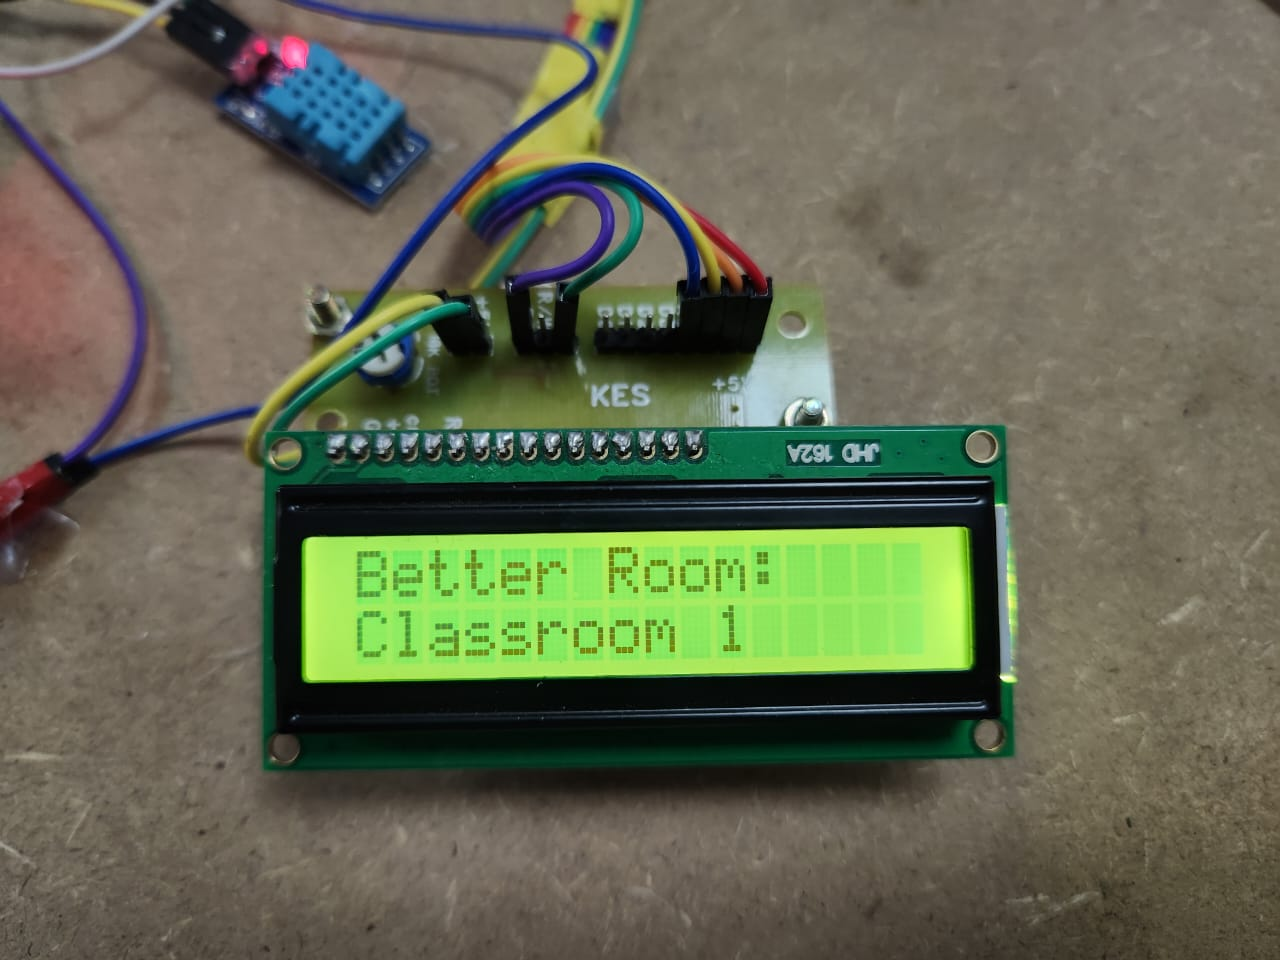
\includegraphics[width=0.8\textwidth]{Chapters/lcd.jpeg}
		\caption{ LCD Output Display Indicating Recommendation of Optimal Classroom}
\end{figure}

As seen on the LCD display connected to the hardware setup, the system is able to provide a real-time recommendation by clearly indicating the better classroom environment at that moment—in this case, "Better Room: Classroom 1". This shows that the system can analyze the environmental quality of both classrooms and provide instant, actionable feedback. The terminal output visible from the Raspberry Pi log shows the real-time readings being collected from both classrooms. These include values for temperature, humidity, CO₂ levels, occupancy, and calculated indicators such as the ventilation quality index (KPIV) and environmental trends. The system collects 120 readings from each classroom, processes them through the LSTM model, and computes a score to determine the better classroom. In the example, Classroom 1 had a score of 61.35, which was significantly better than Classroom 2's score of 114.74, leading to the recommendation of Classroom 1.
\\
\subsubsection{ThingSpeak Integration and Visualization Results}
The ThingSpeak platform successfully integrated the sensor data, creating comprehensive visualizations across multiple channels. As shown in the screenshots, the system effectively managed two separate channels for different classrooms (Classroom 1 and Classroom 2 Environmental Data), each with multiple fields tracking different parameters. The visualization results show clear trends in environmental parameters over time, with interactive charts displaying data from April 13 to April 19. The platform's data export functionality worked seamlessly, allowing for both MATLAB analysis and visualization. The system maintained data integrity with proper timestamping and synchronization across all parameters. The charts effectively displayed both real-time and historical data, providing valuable insights into environmental patterns and trends.

The ThingSpeak platform successfully integrated the sensor data, creating comprehensive visualizations across multiple channels. As shown in the screenshots, the system effectively managed two separate channels for different classrooms (Classroom 1 and Classroom 2 Environmental Data), each with multiple fields tracking different parameters. The visualization results show clear trends in environmental parameters over time, with interactive charts displaying data from April 13 to April 19. The platform's data export functionality worked seamlessly, allowing for both MATLAB analysis and visualization. The system maintained data integrity with proper timestamping and synchronization across all parameters. The charts effectively displayed both real-time and historical data, providing valuable insights into environmental patterns and trends.

\begin{figure}[h!]
		\centering
	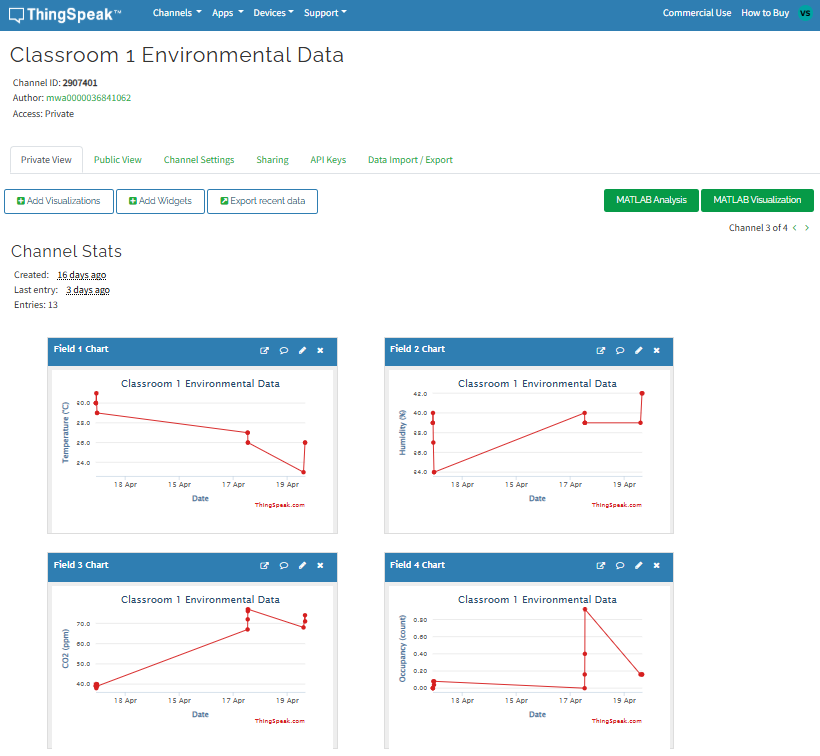
\includegraphics[width=0.8\textwidth]{Chapters/cls1.png}
		\caption{Classroom1 Data}
\end{figure}
The first set of graphs for Classroom 1, the data includes six fields, each visualizing a different environmental or analytical metric over time. Field 1 displays temperature fluctuations, showing a slight decline followed by a rise, indicating responsiveness to occupancy and ventilation control. Field 2 represents humidity, which demonstrates an increasing trend, possibly due to changes in weather or increased occupancy. Field 3 charts CO₂ concentration, where we observe a significant upward trend, peaking around April 17. This correlates with potential occupancy spikes or insufficient ventilation, triggering the system’s predictive and control mechanisms. Field 4 tracks occupancy count derived from IR sensors, which confirms variability in usage patterns. The system successfully captures these changes to make localized decisions. Fields 5 and 6, which show KPIv and trend prediction respectively, remain relatively constant, suggesting early stages of trend stabilization or the need for longer data collection periods to reflect model learning effects.
\begin{figure}[h!]
		\centering
	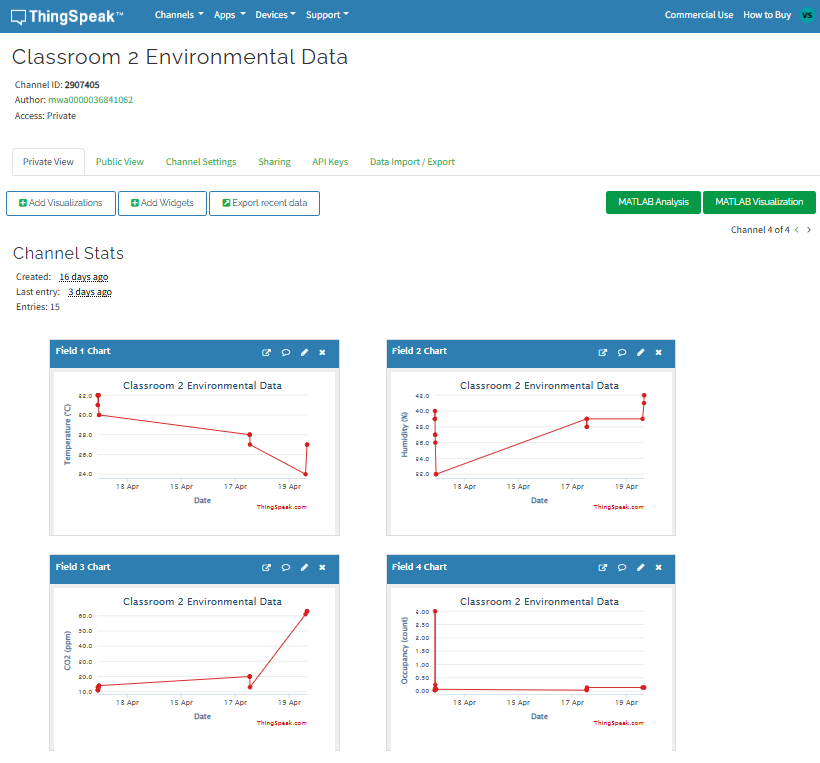
\includegraphics[width=0.8\textwidth]{Chapters/cls2.png}
		\caption{Classroom2 Data}
\end{figure}
\\
The second group of graphs belongs to Classroom 2, with eight fields. Fields 1 to 4 replicate Classroom 1, monitoring temperature, humidity, CO₂ concentration, and occupancy. Field 3 (CO₂ concentration) registers a steep spike, indicating minimal ventilation or more than anticipated occupancy—showing how the system detects declining air quality. Field 4 (occupancy) is low, opening questions on external CO₂ impact or sluggish sensor response. Field 5 through Field 8 are computed KPIv, trend forecasts, model confidence, and model selection history. The values are consistent, with steady predictions, even though some adjustment in real-time model switching would improve performance.



\subsubsection{Certificate Generation system Result}

The certificate generation system proved to be exceptionally good in creating thorough environmental quality assessments. As depicted in the sample certificate, the system was able to effectively process the data obtained to create detailed reports. The certificate indicates a general environmental quality grade of A+ (95/100), out of 6 readings over the given duration. The system accurately computed and displayed average values, indicating temperature at 31.7°C, humidity at 38.0\%, CO2 at 12 ppm, and occupancy at 0.6. The min/max value computation worked exactly, indicating temperature ranges (31.0-32.0°C), humidity ranges (36.0-40.0\%), and CO2 level ranges (11-13 ppm). The KPIv calculation algorithm worked effectively to compute these parameters to calculate the ventilation quality index, which indicated a value of 0.00, meaning perfectly balanced ventilation conditions. The capacity of the certificate generation system to handle several data points and display them in a concise, professional manner reflects the effective use of the environmental monitoring and certification system.
\begin{figure}[h!]
		\centering
	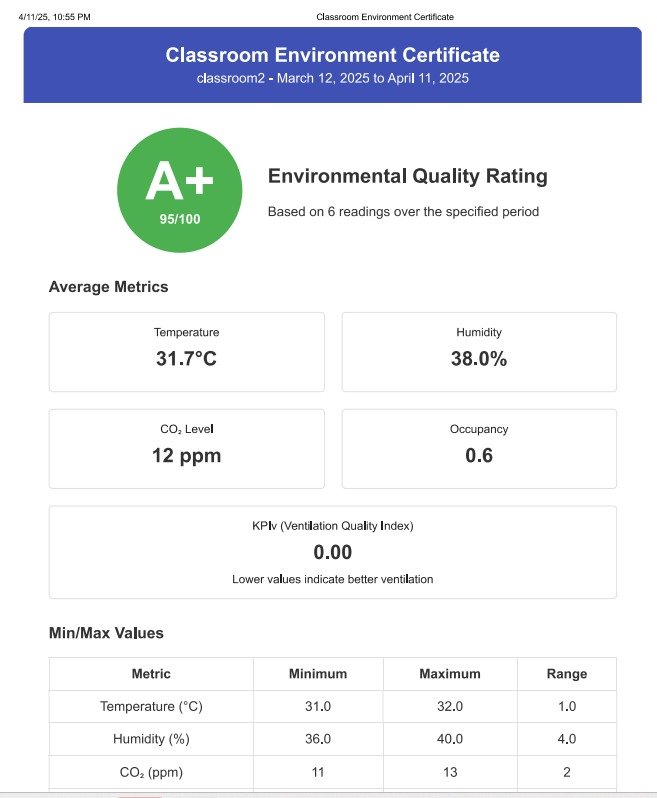
\includegraphics[width=0.8\textwidth]{Chapters/image (4).png}
		\caption{Generated Classroom Environmental Quality Certificate Including KPIV Score}
\end{figure}


